\documentclass[conference]{IEEEtran}
\IEEEoverridecommandlockouts
\usepackage[utf8]{inputenc}
\usepackage[T1]{fontenc}
\usepackage{cite}
\usepackage{amsmath}
\usepackage{graphicx}
\usepackage{booktabs}
\usepackage{array}
\usepackage{tikz}
\usetikzlibrary{positioning,arrows.meta,fit}
\usepackage{url}
\def\UrlBreaks{\do\/\do-\do.\do_}
\begin{document}

\title{Low-Cost TinyML Node for Local Frost Risk Classification and Forecast Validation in Pirgua, Tunja, Colombia\\
{\large Project Proposal}}

\author{\IEEEauthorblockN{Johan Mahomer Le\'on Beltr\'an}
\IEEEauthorblockA{\textit{Data Engineering and Artificial Intelligence}\\
\textit{Universidad Santo Tom\'as}\\
Tunja, Colombia\\
Integrative Project, 2nd semester, term 2026-2}}

\maketitle

\begin{abstract}
Frost damages potato and pasture crops in Boyac\'a, Colombia, and regional forecasts do not describe the microclimate of each farm. This proposal describes a low-cost node in the rural district of Pirgua (Tunja) that measures temperature, humidity and pressure with a BME280 sensor and classifies frost risk on an ESP32-S3 microcontroller with an int8 TensorFlow Lite Micro model. The model reads a 3-hour window stored in a circular buffer and predicts whether the minimum temperature of the next 6 hours will fall to 6\,$^\circ$C (caution) or 2\,$^\circ$C (risk). A periodic web-scraping module stores the public forecast for Tunja in a hash table and compares it with every prediction in a dashboard. The model is trained on an own dataset captured by the node, with a documented protocol and a split by whole days; public data only support the pipeline. Flash, RAM, latency, CPU load and power, measured with an INA219, are reported as percentages and compared with a Raspberry Pi Pico. The firmware, pipeline and scraper already run on both boards with a placeholder model, and the node has logged a full night in Pirgua without a PC.
\end{abstract}

\begin{IEEEkeywords}
edge computing, TinyML, TensorFlow Lite Micro, frost prediction, web scraping, data structures
\end{IEEEkeywords}

\section{Introduction}
Radiative frost occurs on clear, calm nights when the ground and the air near it lose heat quickly, and it damages crops when the air temperature falls near or below 0\,$^\circ$C \cite{fao_frost}. In the Altiplano Cundiboyacense, at about 2\,600--3\,000\,m, these events affect potato, vegetables and pasture. Farmers usually learn about a frost when the damage has already happened, because forecasts are issued per municipality and an official station may be several kilometers away from the field and at a different altitude.

Edge AI makes it possible to run a small classifier next to the sensor, without connectivity or a server. This project integrates three courses: Computer Architecture (device selection and resource measurement), Data Acquisition and Processing (sensor chain, own dataset, model) and Data Structures (a circular buffer on the edge and a hash table in the scraper).

\section{Problem Statement}
According to IDEAM and UPRA, 173\,150\,ha of Boyac\'a were under frost threat in the last week of January 2024, and about 1\,368\,ha of potato were vulnerable in the 19 municipalities analyzed \cite{upra2024}. In February 2020 the price of \textit{papa criolla} in Colombian wholesale markets rose because crops in flower were damaged by frost \cite{dane2020}.

The nearest official station with open data, IDEAM UPTC Tunja (code 2401500086), never recorded 0\,$^\circ$C or less between March 2019 and November 2026; its coldest reading was 0.1\,$^\circ$C and the 1st percentile of its daily minimum is 3.1\,$^\circ$C \cite{ideam_data}. Our hypothesis, to be tested with the node, is that a field in Pirgua is colder than this station, so a local measurement is needed.

\textit{Research question:} can a low-cost embedded node, running a TinyML model locally, classify frost risk in Pirgua and validate that classification against the regional forecast, using only the memory, compute and energy it really needs?

\section{Related Work}
Diedrichs \textit{et al.} predicted frost events with machine learning models trained on data from IoT sensing devices installed in the field \cite{diedrichs2018}. Calder\'on Caro \textit{et al.} published a 30-minute dataset of 23 agricultural stations in the Altiplano Cundiboyacense with frost labels \cite{calderon2026,zenodo2026}. TensorFlow Lite Micro runs neural networks on microcontrollers with a few kilobytes of memory \cite{david2021}, and integer-only quantization reduces the model size and keeps accuracy close to the float model \cite{jacob2018}. Benchmarking embedded ML needs consistent metrics of latency, memory and energy \cite{banbury2020}.

\textit{Gap:} these works either predict frost on a server or study TinyML in general. This project runs the frost classifier on the sensor node in a specific rural district, documents its resource use against a smaller board, and compares each local prediction with the public forecast.

\section{Proposed System}
Fig.~\ref{fig:block} shows the architecture. The node reads the BME280 every 5\,min. Readings are averaged into 30-min steps and pushed into a circular buffer of 6 steps (3\,h). When the buffer is full, the node computes the dew point (Magnus formula \cite{alduchov1996}), encodes the hour of the day as sine and cosine, quantizes the input and runs the model. Every reading and prediction is written to flash (LittleFS) and printed on the serial port. The node sets its clock by NTP over the Wi-Fi available at the site, at boot and again before each reading while the clock is unset, so it works without a PC and recovers after a power cut. On a PC, a listener stores the predictions, a scraper stores the forecast in a hash table every 60\,min, and a Streamlit dashboard shows agreements and disagreements.

\begin{figure}[t]
\centering
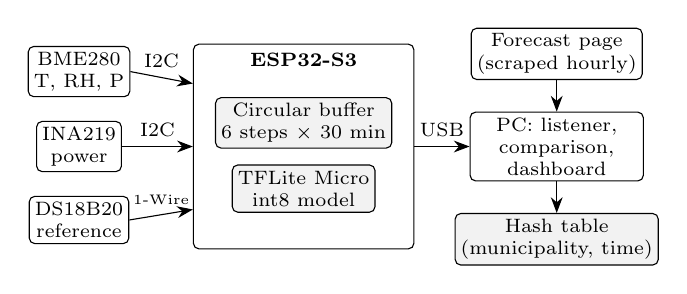
\begin{tikzpicture}[font=\scriptsize, node distance=3mm and 4mm,
 blk/.style={draw, rounded corners=2pt, align=center, minimum height=6mm, inner sep=2pt},
 arr/.style={-{Stealth[length=2mm]}}]
\node[blk] (bme) {BME280\\T, RH, P};
\node[blk, below=of bme] (ina) {INA219\\power};
\node[blk, below=of ina] (ds) {DS18B20\\reference};
\node[blk, right=9mm of ina, minimum width=28mm, minimum height=26mm] (esp) {};
\node[anchor=north, font=\scriptsize\bfseries] at (esp.north) {ESP32-S3};
\node[blk, fill=gray!10] at ([yshift=3mm]esp.center) (buf) {Circular buffer\\6 steps $\times$ 30 min};
\node[blk, fill=gray!10, below=2mm of buf] (tfl) {TFLite Micro\\int8 model};
\node[blk, right=7mm of esp, minimum width=22mm] (pc) {PC: listener,\\comparison,\\dashboard};
\node[blk, above=4mm of pc] (web) {Forecast page\\(scraped hourly)};
\node[blk, below=4mm of pc, fill=gray!10] (hash) {Hash table\\(municipality, time)};
\draw[arr] (bme.east) -- node[above]{I2C} ([yshift=8mm]esp.west);
\draw[arr] (ina.east) -- node[above]{I2C} (esp.west);
\draw[arr] (ds.east) -- node[above, font=\tiny]{1-Wire} ([yshift=-8mm]esp.west);
\draw[arr] (esp.east) -- node[above]{USB} (pc.west);
\draw[arr] (web) -- (pc);
\draw[arr] (pc) -- (hash);
\end{tikzpicture}
\caption{Block diagram. Inference runs on the ESP32-S3; the PC only stores, scrapes and displays.}
\label{fig:block}
\end{figure}

\section{Hardware Architecture}
The edge device is an ESP32-S3 DevKitC-1 (module ESP32-S3-N16R8): two Xtensa LX7 cores up to 240\,MHz with vector instructions, 512\,KB of SRAM, 8\,MB of PSRAM, 16\,MB of flash, and integrated Wi-Fi \cite{esp32s3}. The BME280 and the INA219 share one I2C bus (GPIO8/GPIO9, addresses 0x76 and 0x40) \cite{bme280}; a DS18B20 probe on GPIO4 gives a reference temperature used only for calibration. The INA219 is placed in series with the 5\,V supply, so the measured power includes the board regulator.

\textit{Why not a smaller board:} the more limited alternative is a Raspberry Pi Pico (RP2040: two Cortex-M0+ cores, 264\,KB SRAM, 2\,MB flash, no wireless) \cite{rp2040}; the Arduino core used runs it at 200\,MHz. It runs the same int8 model with the same TensorFlow Lite Micro library and the same benchmark, so both reports can be compared (Table~\ref{tab:res}). The Pico has no Wi-Fi, so it cannot recover its clock by NTP after a power cut, and the model uses the hour of the day as input; this is a functional reason in favor of the ESP32-S3. The ESP32-S3 was adopted on the recommendation of the course instructor, Prof. Fernando Jim\'enez, and the measurements of Table~\ref{tab:res} quantify how much of it the task really uses. \textit{Why not a larger one:} a single-board computer would add cost and power without any benefit for a dense model of a few kilobytes.

\section{Data Acquisition and Dataset}
Table~\ref{tab:protocol} summarizes the capture protocol. The BME280 runs in forced mode with oversampling $\times$1 and the filter off, so it sleeps between readings and does not heat itself. Readings outside the datasheet range are stored with status \texttt{sensor\_error} and excluded later. The BME280 and the DS18B20 are installed together in the sun shield, so their offset is measured in place during the capture; it is applied when the dataset is built, never to the raw files.

\textit{First night.} On 20--21 November 2026 the node ran about 14\,h in Pirgua without a PC: 170 readings, all valid, one every 5\,min with no gaps or restarts, clock set by NTP. However, the BME280 was left inside the electronics box and only the probe was outside. At night the BME280 read 4.4\,$^\circ$C more than the probe (standard deviation 0.4\,$^\circ$C, against $+0.09$\,$^\circ$C when both shared the same air indoors) and about 60\,\% humidity, while the outdoor air, at the probe temperature, had about 80\,\%. The night is kept as a test and not used; both sensors now go outside the box, together in the sun shield. The outdoor minimum was 12.5\,$^\circ$C, so there was no frost risk.

\begin{table}[t]
\caption{Capture protocol (draft)}
\label{tab:protocol}
\centering
\begin{tabular}{@{}>{\raggedright}p{2.2cm}>{\raggedright\arraybackslash}p{5.6cm}@{}}
\toprule
Parameter & Value \\
\midrule
Site & Pirgua, Tunja (author's home); 1.5\,m above ground; BME280 and probe together in a sun shield, outside the electronics box \\
Period & November to February (cold season) \\
Sampling & Every 5\,min; averaged into 30-min steps \\
Stored row & time (UTC$-$5), T, RH, P, reference T, status \\
Clock & NTP over the home Wi-Fi at every boot; \texttt{SETTIME} from a PC as fallback \\
Label & minimum T of the next 6\,h: risk $\le$2\,$^\circ$C, caution $\le$6\,$^\circ$C, else no risk \\
Split & 70/15/15 by whole days, stratified by the highest class of each day, fixed seed \\
Versions & v1, v2, \dots; never overwritten \\
\bottomrule
\end{tabular}
\end{table}

\textit{Labeling.} The class of a window depends on the minimum air temperature of the next 6\,h: \emph{risk} if it is at or below 2\,$^\circ$C, \emph{caution} if it is at or below 6\,$^\circ$C, and \emph{no risk} otherwise. The sensors are at 1.5\,m, and on clear, calm nights the crop surface can be several degrees colder than the air at that height \cite{fao_frost}, so 2\,$^\circ$C in the air is treated as possible frost on the crop. The 6\,$^\circ$C limit is an operational caution band, not an agronomic value: nights at or below 2\,$^\circ$C are rare (9 days at the UPTC station in 2019--2026), and the band gives the model examples of cold nights. Both limits are parameters, and a minimum of 10 training days per class is required before training.

\textit{Leakage.} Every reading of a day falls in the same split, for all sources, so no day is shared between train, validation and test; days are split separately by their highest class, so the rare cold days also reach validation and test. Public data (IDEAM UPTC Tunja \cite{ideam_data} and the Altiplano dataset \cite{zenodo2026}, with station 11 removed because of a faulty sensor) are used only to develop the pipeline; the final model is trained and evaluated with node data.

\textit{Ethics.} No personal data is collected; the node is installed with the permission of the landowner.

\section{Data Structures}
Table~\ref{tab:ds} gives the two structures, both written without libraries.

\textit{Circular buffer (edge).} A fixed array of $n=6$ steps and a \texttt{head} index that wraps around. Insertion overwrites the oldest step. A shifting array would cost $O(n)$ per insertion, and a linked list needs dynamic memory that can fragment the heap of a microcontroller.

\textit{Hash table (scraper).} Buckets with chaining, an own polynomial hash of the key (municipality, date, hour), and doubling when the load factor exceeds 0.75. For $m$ lookups over $n$ forecasts, a list of pairs costs $O(mn)$ and the table $O(m)$ on average.

\begin{table}[t]
\caption{Data structures and complexity}
\label{tab:ds}
\centering
\begin{tabular}{@{}lll@{}}
\toprule
Structure & Operation & Time \\
\midrule
Circular buffer & push, get($i$), size & $O(1)$; memory $O(n)$ fixed \\
Hash table & put, get, remove & $O(1)$ avg., $O(n)$ worst \\
 & resize & $O(n)$, amortized $O(1)$ \\
\bottomrule
\end{tabular}
\end{table}

\section{Methodology and Work Plan}
\textit{Model.} Input: 6 lags of temperature, humidity, dew point and (if available in every source) pressure, plus hour sine and cosine (20 or 26 inputs). Network: dense 16--8--softmax with class weights for imbalance, early stopping (patience 5). Full int8 post-training quantization calibrated with 500 training rows \cite{jacob2018}. The F1 of the int8 model is compared with the float model on the same test split (R3), and the node output is compared with the PC int8 model on 100 test vectors and on 50 raw windows; with the placeholder model both boards gave exactly the same output as the PC in every case.

\textit{Scraping.} The forecast page of Tunja (wttr.in) is scraped every 60\,min with retries and an error log; IDEAM publishes its forecast only as map applications and bulletins. Its known limit is that it gives no values before sunrise, when the daily minimum occurs; such predictions are shown as not comparable.

\textit{Phases.} (1) Definition and proposal, 1 week; (2) design, 1 week; (3) implementation, 0.5 week; (4) tests and measurements, 0.5 week; (5) report and defense, 1 week. Capture starts as early as possible because it is the slowest step.

\textit{Risks.} The main risk is that the node records no night at or below 2\,$^\circ$C during the capture; it will be reported, and the script warns when any class has fewer than 10 training days. Other risks are power cuts without Wi-Fi, which stop logging until the clock is set again, and the limits of the forecast source.

\section{Expected Resource Usage}
Table~\ref{tab:res} shows a pipeline test on both boards with the same \textit{placeholder} model (20 inputs, 16--8 units, 2 classes, provisional threshold), measured on 20 November 2026. These are not project results; they show that the measurement works and the order of magnitude. Final values, including power and energy per inference, will be measured with the real model. With this model both boards stay far below the 30\,\% limit, and the latency is negligible against the 30-min period between inferences; the Pico is about 1.7 times slower but would still be sufficient. The program sizes are not equivalent: the ESP32-S3 firmware also reads the sensors, logs to flash and uses Wi-Fi, while the Pico firmware only runs the benchmark. The choice of the ESP32-S3 therefore rests on its Wi-Fi (clock without a PC and, as future work, an alert to the farmer's phone) and on the margin for the final model, to be confirmed with the power measurements.

\begin{table}[t]
\caption{Pipeline test, placeholder model (\% of the total in parentheses)}
\label{tab:res}
\centering
\footnotesize
\begin{tabular}{@{}lrr@{}}
\toprule
Metric & ESP32-S3 (240\,MHz) & Pico (200\,MHz) \\
\midrule
Latency, 200 runs & 0.050 $\pm$ 0.016 ms & 0.087 $\pm$ 0.022 ms \\
Tensor arena & 876 B (5.4) & 964 B (5.9) \\
Model & 3.2 kB (0.02) & 3.2 kB (0.15) \\
Program & 476 kB (36.3\textsuperscript{a}) & 156 kB (7.4) \\
Heap & 52 kB peak (14.2) & 2.3 kB in use (1.0) \\
Stack, peak & 2.5 kB (30.9) & -- \\
Same output as PC & 100/100, 50/50 & 100/100 \\
Power & not measured yet & not measured yet \\
\bottomrule
\multicolumn{3}{@{}l}{\textsuperscript{a}\,of the 1.25\,MB program partition; 2.8 of the 16\,MB flash.}
\end{tabular}
\end{table}

The cycle counter of each core gives the CPU cycles per inference, and the CPU load is estimated as mean latency divided by the 30-min period between inferences; power is the INA219 average of 50 readings at idle and during continuous inference, and energy per inference is power times latency.

\section{Expected Outcomes}
(1) A working node that logs and predicts in Pirgua, shown live or in a video of up to 5 minutes; (2) a versioned own dataset with its capture protocol; (3) a float and an int8 model with their F1 comparison; (4) a resource report of the ESP32-S3 against the Raspberry Pi Pico; (5) a dashboard comparing local predictions with the forecast; (6) the final IEEE report and the public repository \url{https://github.com/MahomerLeon/frost-node-tinyml}.

\begin{thebibliography}{00}
\bibitem{fao_frost} R. L. Snyder and J. P. de Melo-Abreu, \textit{Frost Protection: Fundamentals, Practice and Economics}, vol.~1, Environment and Natural Resources Series no.~10. Rome, Italy: FAO, 2005.
\bibitem{upra2024} IDEAM and UPRA, ``Cultivos y \'areas vulnerables a las heladas en enero de 2024,'' Bogot\'a, Colombia, 2024. [Online]. Available: \url{https://upra.gov.co/es-co/Documents/fenomeno_nino/20240125_Heladas-Enero-2024.pdf}
\bibitem{dane2020} DANE--SIPSA, ``Informe de mercados, semana del 8 al 14 de febrero de 2020,'' Bogot\'a, Colombia, Feb. 2020. [Online]. Available: \url{https://www.dane.gov.co/files/investigaciones/agropecuario/sipsa/heladas/informe-heladas-14-feb-2020.pdf}
\bibitem{ideam_data} IDEAM, ``Datos hidrometeorol\'ogicos crudos: temperatura, humedad y presi\'on, estaci\'on UPTC Tunja 2401500086,'' datos.gov.co, datasets sbwg-7ju4, uext-mhny and 62tk-nxj5. Accessed: Nov. 5, 2026.
\bibitem{diedrichs2018} A. L. Diedrichs, F. Bromberg, D. Dujovne, K. Brun-Laguna, and T. Watteyne, ``Prediction of frost events using machine learning and IoT sensing devices,'' \textit{IEEE Internet Things J.}, vol.~5, no.~6, pp.~4589--4597, 2018, doi: 10.1109/JIOT.2018.2867333.
\bibitem{calderon2026} E. Calder\'on Caro, D. A. Casta\~neda S\'anchez, J. R. Ballesteros, and J. W. Branch-Bedoya, ``Topoclimatic graph dataset for frost prediction in the tropical high-mountain Altiplano Cundiboyacense, Colombia,'' \textit{Data}, vol.~11, no.~8, Art. no.~205, 2026, doi: 10.3390/data11080205.
\bibitem{zenodo2026} E. Calder\'on Caro \textit{et al.}, ``Topoclimatic Graph Dataset for Frost Prediction,'' v1.0, Zenodo, 2026, doi: 10.5281/zenodo.20616866.
\bibitem{david2021} R. David \textit{et al.}, ``TensorFlow Lite Micro: Embedded machine learning for TinyML systems,'' in \textit{Proc. Mach. Learn. Syst. (MLSys)}, vol.~3, 2021, pp.~800--811.
\bibitem{jacob2018} B. Jacob \textit{et al.}, ``Quantization and training of neural networks for efficient integer-arithmetic-only inference,'' in \textit{Proc. IEEE Conf. Comput. Vis. Pattern Recognit. (CVPR)}, 2018, pp.~2704--2713.
\bibitem{banbury2020} C. R. Banbury \textit{et al.}, ``Benchmarking TinyML systems: Challenges and direction,'' arXiv:2003.04821, 2020.
\bibitem{alduchov1996} O. A. Alduchov and R. E. Eskridge, ``Improved Magnus form approximation of saturation vapor pressure,'' \textit{J. Appl. Meteorol.}, vol.~35, no.~4, pp.~601--609, 1996.
\bibitem{esp32s3} Espressif Systems, ``ESP32-S3 Series Datasheet.'' [Online]. Available: \url{https://www.espressif.com/sites/default/files/documentation/esp32-s3_datasheet_en.pdf}
\bibitem{rp2040} Raspberry Pi Ltd., ``RP2040 Datasheet.'' [Online]. Available: \url{https://datasheets.raspberrypi.com/rp2040/rp2040-datasheet.pdf}
\bibitem{bme280} Bosch Sensortec, ``BME280 Combined humidity and pressure sensor, Datasheet.''
\end{thebibliography}

\end{document}
